\section{Methodology}

\subsection{The Data2MCP Architecture}

The \textsc{Data2MCP} framework is designed for open-ended analytical queries that require sequential tool dispatch and multi-source synthesis. Formally, given a natural language query $q$ and a set of Model Context Protocol (MCP) tools $\mathcal{T} = \{t_1, t_2, \dots, t_n\}$, where each tool encapsulates an underlying data source, the system produces a final textual response via a multi-turn reasoning loop. 

\begin{figure*}[t]
  \centering
  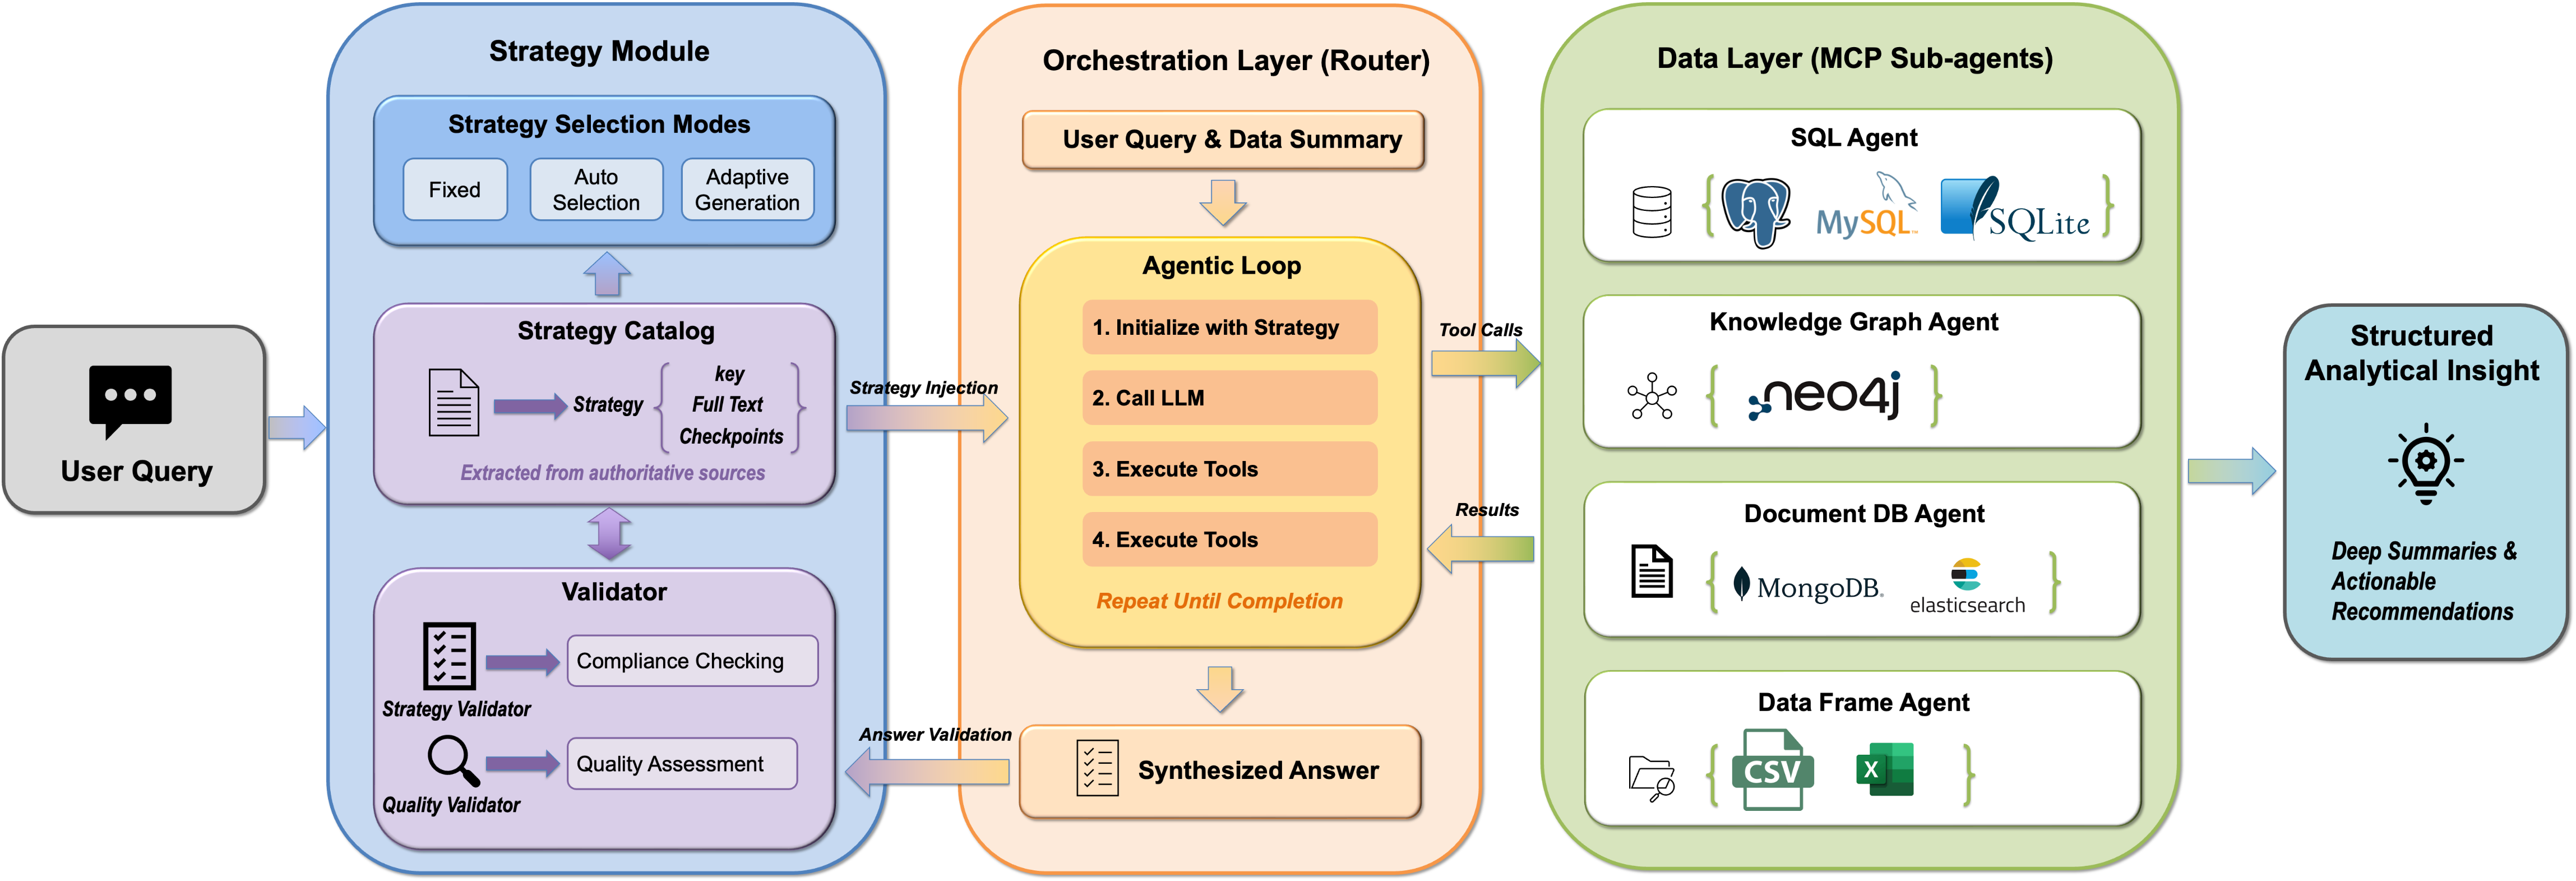
\includegraphics[width=0.98\textwidth]{figures/system_overview.png}
  \caption{Data2MCP system architecture. The Strategy Module (left) selects or generates a specific analytical methodology to be embedded into the controller context. The Router (center) executes the multi-turn agentic execution loop, dispatching programmatic calls to MCP sub-agents (right). Compliance is evaluated post-execution by the Strategy and Output Validators.}
  \label{fig:architecture}
\end{figure*}

To manage source heterogeneity and enforce systematic reasoning paths, the framework decouples execution into three distinct operational layers (Figure~\ref{fig:architecture}): a data layer for interface encapsulation, an orchestration layer (Router) for multi-turn execution, and a strategy layer for procedural methodology injection and validation.

\paragraph{Data Layer: Interface Abstraction.}
The data layer unifies disparate data modalities under a standardized MCP interface, allowing the central controller to interact with different database engines using a single tool-calling protocol. The current implementation supports four data source categories: 
(1) Relational Databases, accessed via read-only Text-to-SQL (SQLAlchemy) capped at 1,000 rows per query; 
(2) Knowledge Graphs, queried via Text-to-Cypher (Neo4j) with a maximum return of 500 records; 
(3) Unstructured Document Collections, managed via FAISS vector retrieval ($top\text{-}k=5$, chunk size of 1,000 characters); and 
(4) Tabular Data, manipulated through localized Pandas DataFrame operations.

Every tool within this layer exposes an invariant interface: a natural-language description, a JSON-schema parameter definition, and a textual response limited to a 10,000-character budget. This uniformity removes source-specific routing logic from the orchestration layer; the central LLM selects tools based entirely on semantic descriptions, rendering the Router source-agnostic. The 10,000-character cap prevents context window overflow during extended execution sequences. Truncation is handled by appending an explicit metadata flag to the relevant content prefix. Read-only permissions are enforced natively at the database level rather than via system prompts, ensuring data integrity independent of model stochasticity.

\paragraph{Orchestration Layer: Multi-Turn Execution Loop.}
The Router coordinates the execution loop across sequential steps. At turn $t$, the Router provides the core LLM with: (i) the accumulated conversation history $H_{<t}$, (ii) the tool definitions $\mathcal{T}$, and (iii) the strategy specification $\mathcal{S}$ embedded in the controller context. The Router parses the model output, executes the designated tool calls, appends the results as tool-role messages to update the history to $H_t$, and repeats this sequence until the model invokes the end\_with\_message utility or hits a maximum execution budget of 30 turns.

The 30-turn budget serves as a practical ceiling to bound execution costs, as empirical returns diminish beyond this threshold. The end\_with\_message tool acts as a deterministic constraint that prevents silent failures; it prevents the model from terminating execution without outputting a synthesized final narrative. To handle network and database instabilities, failed tool invocations are retried once using an exponential backoff schedule. If the second attempt fails, the execution log captures the error as a standard tool response, forcing the controller to adapt its planning trajectory without the requested evidence.

\subsection{Structured Strategy Injection}

Agent execution failures are frequently caused by suboptimal analytical workflows, such as omitting data verification steps or ignoring conflicting evidence. We mitigate this behavioral drift by injecting structured "analysis playbooks" into the Router's controller context to constrain execution pathways without restricting the specific content of individual tool calls.

\paragraph{StrategySpec: Formalizing Procedural Constraints.}
An analytical methodology is formalized as a StrategySpec tuple $\langle k, \tau, \mathcal{C} \rangle$, where $k$ is a unique identifier, $\tau$ is the guidance string consisting of 2--6 procedural sentences injected verbatim into the prompt, and $\mathcal{C}$ is a set of explicit behavioral checkpoints. 

This three-field formulation separates the operational instruction from the evaluation criterion. While $\tau$ functions as an active constraint on the LLM's generation loop, $\mathcal{C}$ serves as the reference ground truth for automated compliance validation. Restricting $\tau$ to 2--6 sentences minimizes instruction distraction, ensuring that methodology injection does not degrade the model's adherence to the core task prompt.

\begin{table}[h]
  \centering
  \small
  \caption{Example of a StrategySpec instance for the Analysis of Competing Hypotheses (ACH) methodology.}
  \label{tab:strategyspec}
  {\setlength{\tabcolsep}{3pt}\begin{tabular}{p{1.8cm}p{4.7cm}}
    \toprule
    \textbf{Field} & \textbf{Content} \\
    \midrule
    \texttt{key} & \texttt{ach} \\
    \texttt{full\_text} & Identify all plausible hypotheses. Search for diagnostic evidence that can discriminate between them. Evaluate each hypothesis against the gathered evidence. Methodically eliminate inconsistent hypotheses. Synthesize the final conclusion with explicit uncertainty levels. \\
    \texttt{checkpoints} & \{hypothesis\_enumeration, evidence\_matrix, elimination\_step, uncertainty\_statement\} \\
    \bottomrule
  \end{tabular}}
\end{table}

\paragraph{Catalog Construction and Selection Modes.}
The framework maintains a permanent catalog of $|\mathcal{S}|=74$ strategies. This includes 70 methodologies automatically parsed from domain texts~\cite{heuer2010structured, crispdm2000} using an offline LLM extraction pipeline (Appendix~\ref{app:extraction}). The catalog scale is bounded to guarantee that the full option space can be processed within a single selection prompt without exceeding context limitations.

The framework supports three discrete operational selection modes: (1) Fixed Mode, where a user specifies a target key $k$ and its corresponding $\tau$ is loaded; (2) Auto-selection Mode, where a lightweight LLM call matches the incoming query $q$ against the strategy catalog using a brief data summary; and (3) Adaptive Generation Mode, where the system dynamically assembles a custom StrategySpec based on query intent and data dimensionality.

\paragraph{Closed-Loop Compliance Validation.}
Verifying adherence to an injected methodology requires an explicit feedback loop. We implement a two-stage validation mechanism that produces a normalized compliance score in the range $[0, 1]$:
(1) The StrategyValidator continuously evaluates execution trace statistics, measuring physical metrics such as parallel-call ratios and tool invocation diversity against strategy-specific thresholds.
(2) The OutputValidator conducts a post-hoc evaluation of the final narrative answer to confirm that all specified elements in checkpoints $\mathcal{C}$ are satisfied.

Empirical evaluation indicates that this compliance score reflects execution quality rather than prompt formatting alignment; compliance correlates significantly with final answer correctness (Pearson $r=0.34$, $p<0.001$). When execution falls below threshold compliance, the system outputs a structured warning containing checkpoint-level failures, isolating which analytical procedures were bypassed.

\paragraph{Architectural Modularity.}
In summary, the three-layer design of Data2MCP addresses distinct orthogonal axes of the analysis task. The data layer standardizes access to heterogeneous storage systems; the orchestration layer drives sequential reasoning execution; and the strategy layer enforces methodological rigor via structural constraints and verification. This modularity isolates each component, permitting independent additions of tools, strategies, or validators without altering the core framework logic.